\section{Reproducibility within the context of energy}\label{sec:benchmarking_reproducibility}
\subsection{Introduction}

Empirical measurements are critical to capture the effect of developers' choices on software energy consumption.
To accomplish this, one should not overlook the benchmarking pitfalls highlighted in the state of the art~\cite{van_der_kouwe_benchmarking_2018}.

Second, one should not ignore tremendous progress in computer science, which have led to a rise in the number of obsolete results.
Furthermore, when it comes to comparative research, the execution environment may have an impact on the study itself.
Finally, between the exploratory experiment and the publication of the results, new candidates may have emerged and others may have changed.

As a result, it is critical not only to ensure that the results can be "reproduced", so one can test their hypothesis in different environments, but also to provide room for new candidates.
In this section, we will address these issues and investigate several ways of encapsulating the systems-under-test to ensure experiment reproducibility in the context of energy consumption tests while providing the benefits and drawbacks of each strategy.
Later in this section, we will also propose a protocol to ensure that the results are not only reproducible but extensible.

% Furthermore, when it comes to evaluating the energy consumption of software, other challenges occur, such as the impact of hardware, the difference between the machines used for measurements and those that may apply the results, and so on.
% Regarding the "representativeness" of the benchmarks, we will elaborate in the section entitled Perspectives.
%% this is might be the part that treats reproducibility for my case 



%%%%%%%%% preliminary taughts and section structure 
% The need of reproducibility in our field - software optimization based on empirical studies -

% The importance of Virtualisation for reproducibility \cite{howe_virtual_2012}
% some of the most important parts are
% - fewer constraints on research methods
% - on-demand backups
% - virtual Machines as Publications
% - more Variables captured



%%%% part of the state of the art 
% In the area covered by this PhD thesis, reproducibility might be achieved by ensuring the same execution settings of physical nodes, virtual machines, clusters or cloud environments.
%%% why it won't work for energy consumption 
% However, when it comes to measuring the energy consumption of a system, applying acknowledged guidelines and carefully repeating the same benchmark can nonetheless lead to different energy footprints not only among homogeneous nodes, but even within a single node.
%% reseasons why 
% One major problem that hinders the reproducibility of the empirical benchmarks is the interaction with the external environment, either as concurrency or dependencies.
% Therefore, researchers cannot observe the same results, unless they duplicate the same environment.


% \begin{itemize}
%     \item textbf{expermimental protocol}: Which describes, the context and  an orchestrator that handles the experiment, this orchestrator should take as an entry 
%     \item \textbf{candidates}: a set of candidates that will be used in the experiment. The candidates should be agnostic of the experiment context and they all
% \end{itemize}

% Now that we have covered the general strucutre of the protocol, this section details the specific aspects of the protocol that are relevant to the energy consumption analysis.
% We will first discuss how to insure the extension of the candidates. later we will talk about the energy metrics and how to ensure the accuracy when it comes to the measurement of the energy consumption.


\subsection{Virtual Machines}
The very first choice should be to use \emph{Virtual Machines} (VM), which allow researchers to select the most appropriate tools, software, and operating system that they are most comfortable with without incurring the cost of changing the actual working environment, giving them more control over dependencies and the execution environment.
Furthermore, adopting a VM addresses the \emph{replication crisis} since virtual images allow even the most sophisticated architecture to be simply replicated by instantiating a copy of the image.

This option, however, comes at a cost. Because of the hypervisor, software will be built on two kernels: one for the virtual machine (guest) and one for the host machine, resulting in a visible overhead and a negative influence on the performance of the system-under-test.
As a result, we cannot use VM for performance-related tests.
Isolation is another drawback of VM: while this feature protects the experimental setting from unwanted interference from the outside world, it is possible that this interaction is required—-especially if the experiment is dependent on an external source such as energy monitors.

\subsection{Containers}
Another option would be to use something that allows us to benefit from the host OS's isolation while simultaneously simplifying replication as proposed by VM and the direct interface with the hardware provided by the traditional techniques.

Containers provide such an advantage by ensuring application separation and ease of replication.
Figure~\ref{environement:virtualization_technique} depicts the architectural differences between virtualization and container technologies. There are three main types of virtualization.
\begin{itemize}
    \item \textsf{Type\,1}: runs on the hardware directly.
          It is primarily utilized by cloud providers where there is no host OS and only VMs that run on the open-source Xen or VMware ESX hypervisors.

    \item \textsf{Type\,2}: runs on top of the host operating system and is most commonly found on personal computers. VMware server and virtualBox are notable examples of this category, and most researchers' experiments use them.
          However, because of the two operating systems, the applications are typically slower.

    \item \textsf{Containers}: run their operating systems on the host kernel rather than their own , which makes them smaller, faster, and more efficient in terms of hardware utilization. One can cite \emph{Docker}, \emph{Linux LXC}, or \emph{LXD}~\cite{abuabdo_virtualization_2019}.
\end{itemize}


\begin{figure}
    \center{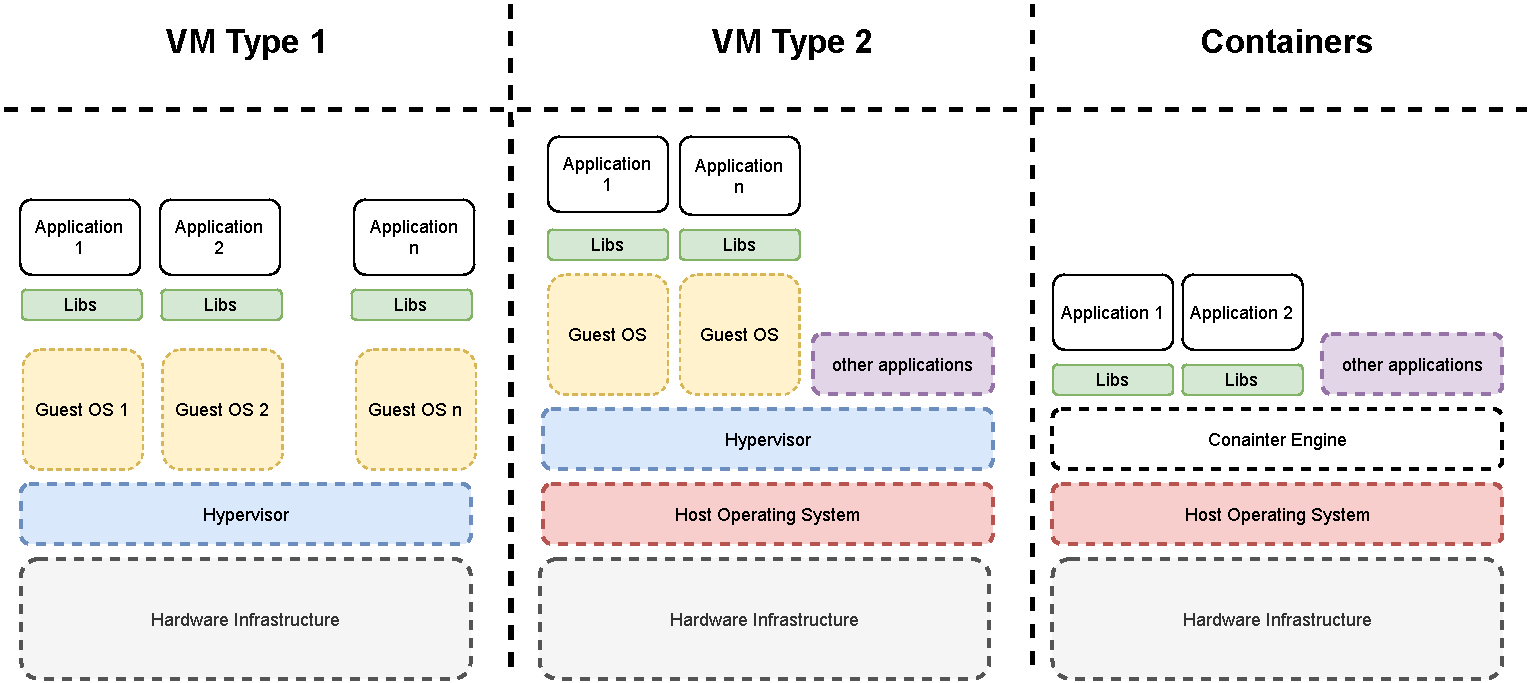
\includegraphics[width=1\linewidth]{imgs/virtualization_techniques}}
    \caption{Different Methods of Virtualization}\label{environement:virtualization_technique}
\end{figure}


\subsection{Docker Vs. Virtual Machine}
Despite the fact that Type 1 is more performant than Type 2, the latter is the most used in research, as most researchers tend to conduct their experiments on their own machines. Docker, on the other hand, is the most well-known container technology. In our case, we are more likely to promote Docker for two reasons:
\begin{enumerate}
    \item As previously stated in literature~\cite{van2016power,morabito_power_2015}, we require a lightweight orchestrator to limit the overhead on energy usage of our experiments
    \item We need to communicate with the host OS because we are using hardware sensors to measure the energy consumption.
\end{enumerate}

% A special notice to \href{https://github.com/powerapi-ng/virtualwatts}{virtualwatts}. A framework that enables us to retrieve the energy consumption of a virtual machine.


\subsection{Docker \& Energy}
Now that we have decided to use container technology to enclose our tests, what effect will this have on the amount of energy consumed by our tests ?
%%%%%%%%%


Using research from \cite{eddie_antonio_santos_how} who examined how adding the Docker layer affected energy consumption, \citeauthor{eddie_antonio_santos_how} conducted their experiment by running numerous benchmarks both with and without Docker. They contrasted the energy usage and execution time that resulted.
The first step was to observe the effects of the orchestrator and the Docker deamon while there was no work to be done.
Then, they use three benchmarks in their experiments: Wordpress, Reddis and PostgreSQL.
The values below show the system under test's energy consumption while it is idle.
Docker has an overhead of roughly $1,000$  joules, as seen in Figure~\ref{fig:docker_idle} .


\begin{figure}
    \center{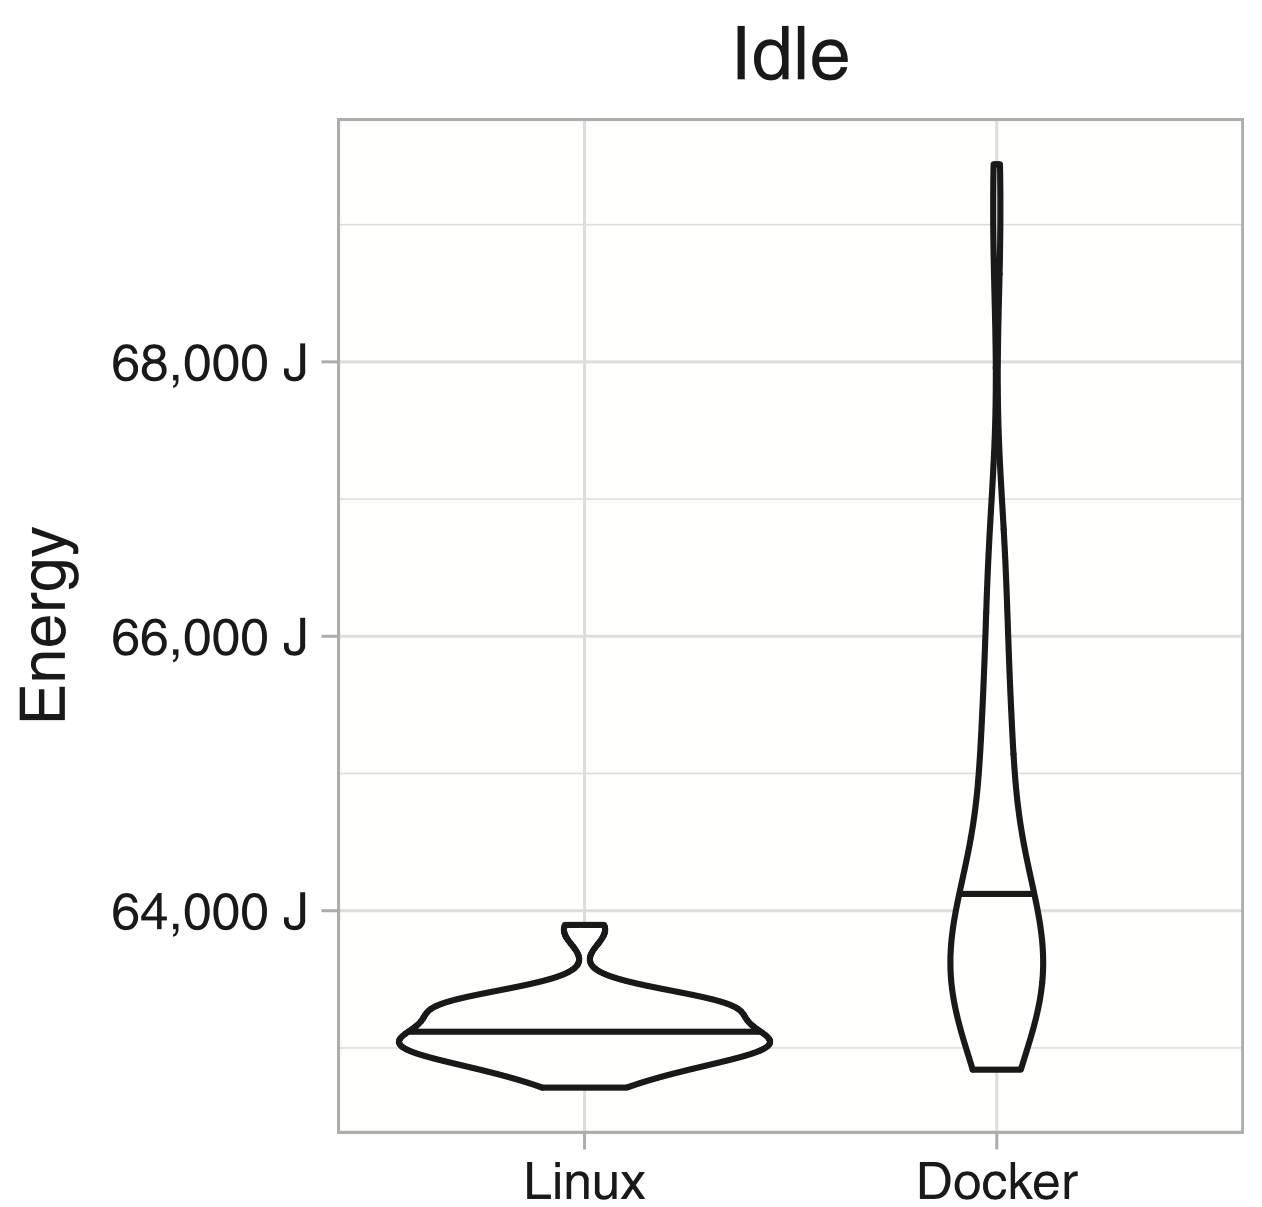
\includegraphics[width=.5\linewidth]{imgs/docker_vs_vm_energy_paper/idle_energy}}
    \caption{energy consumption of Idle system with and without docker \cite{eddie_antonio_santos_how}}\label{fig:docker_idle}
\end{figure}

Yet, as seen in Figure~\ref{fig:docker_reddis}, Docker increased the execution duration of the benchmark by 50 seconds, which led to a significant rise in the energy usage.
According to the authors, this overhead is primarily caused by the Docker daemon and not by the fact that  the application is in a container.


Furthermore, they calculated the cost of this extra energy, which was less than 0.15\$ in the worst-case scenario, which is insignificant in comparison to the benefits of Docker for isolation and reproducibility.

To summarize, Docker-based software tends to consume more energy since it takes longer to execute.
The execution of the Docker daemon causes an increase in average power consumption of only \textbf{2\,Watts}.
This overhead can reach up to 5\% in IO-intensive applications, while it is barely visible in CPU- or DRAM-intensive workloads.

\begin{figure}[!bht]
    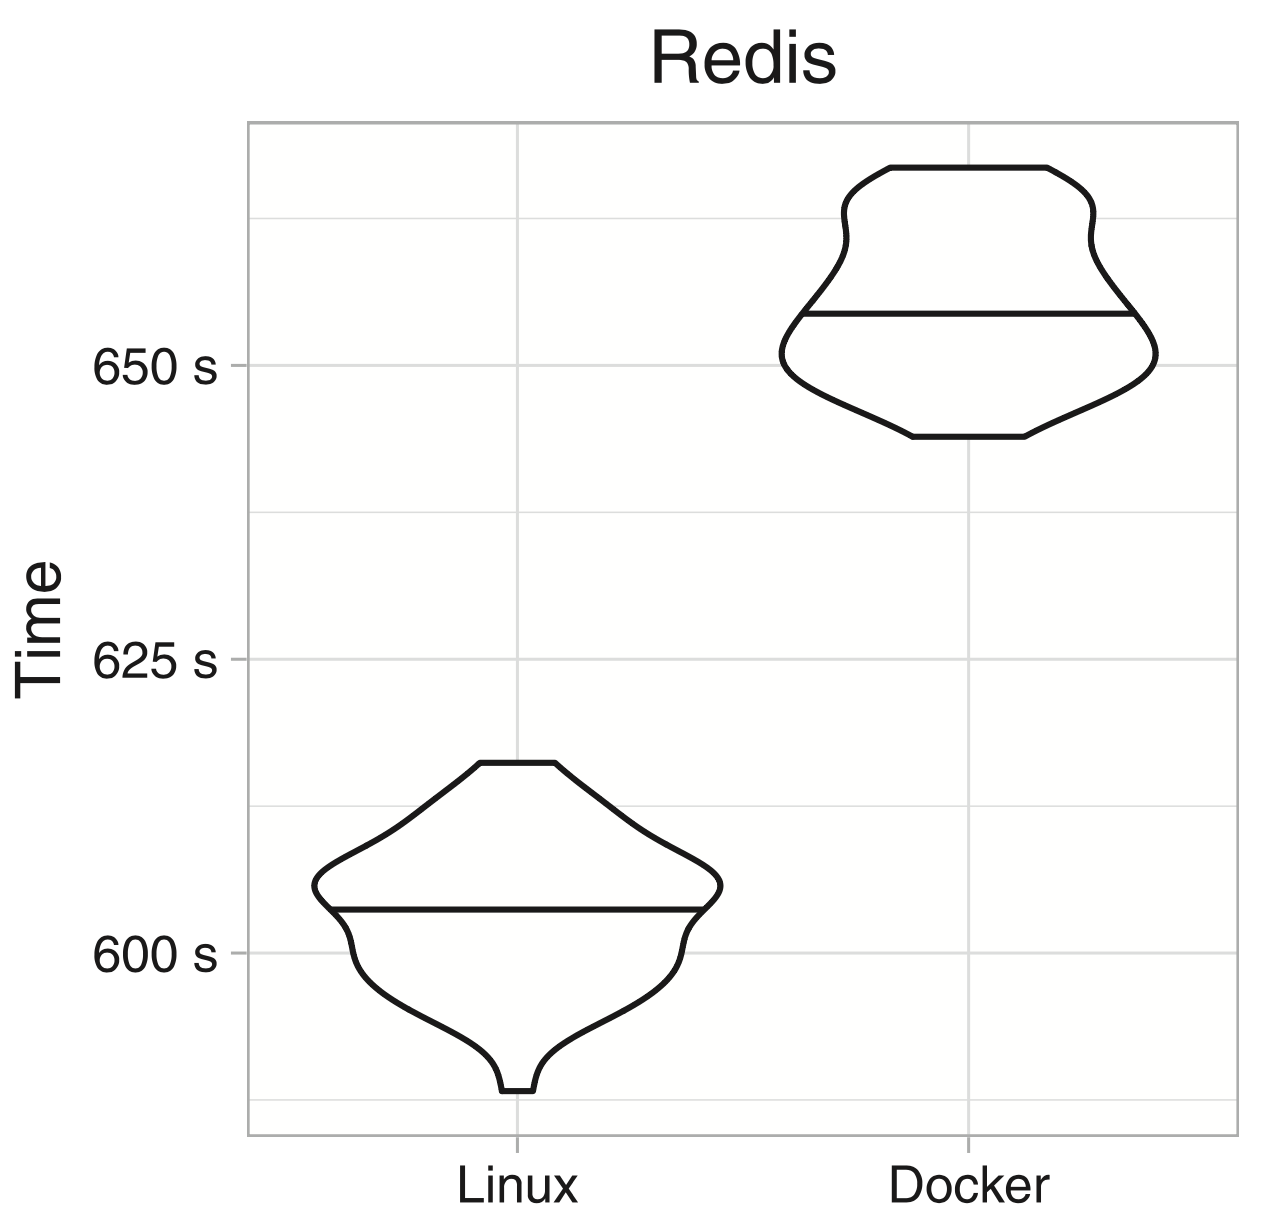
\includegraphics[width=.5\linewidth]{imgs/docker_vs_vm_energy_paper/reddis_time}
    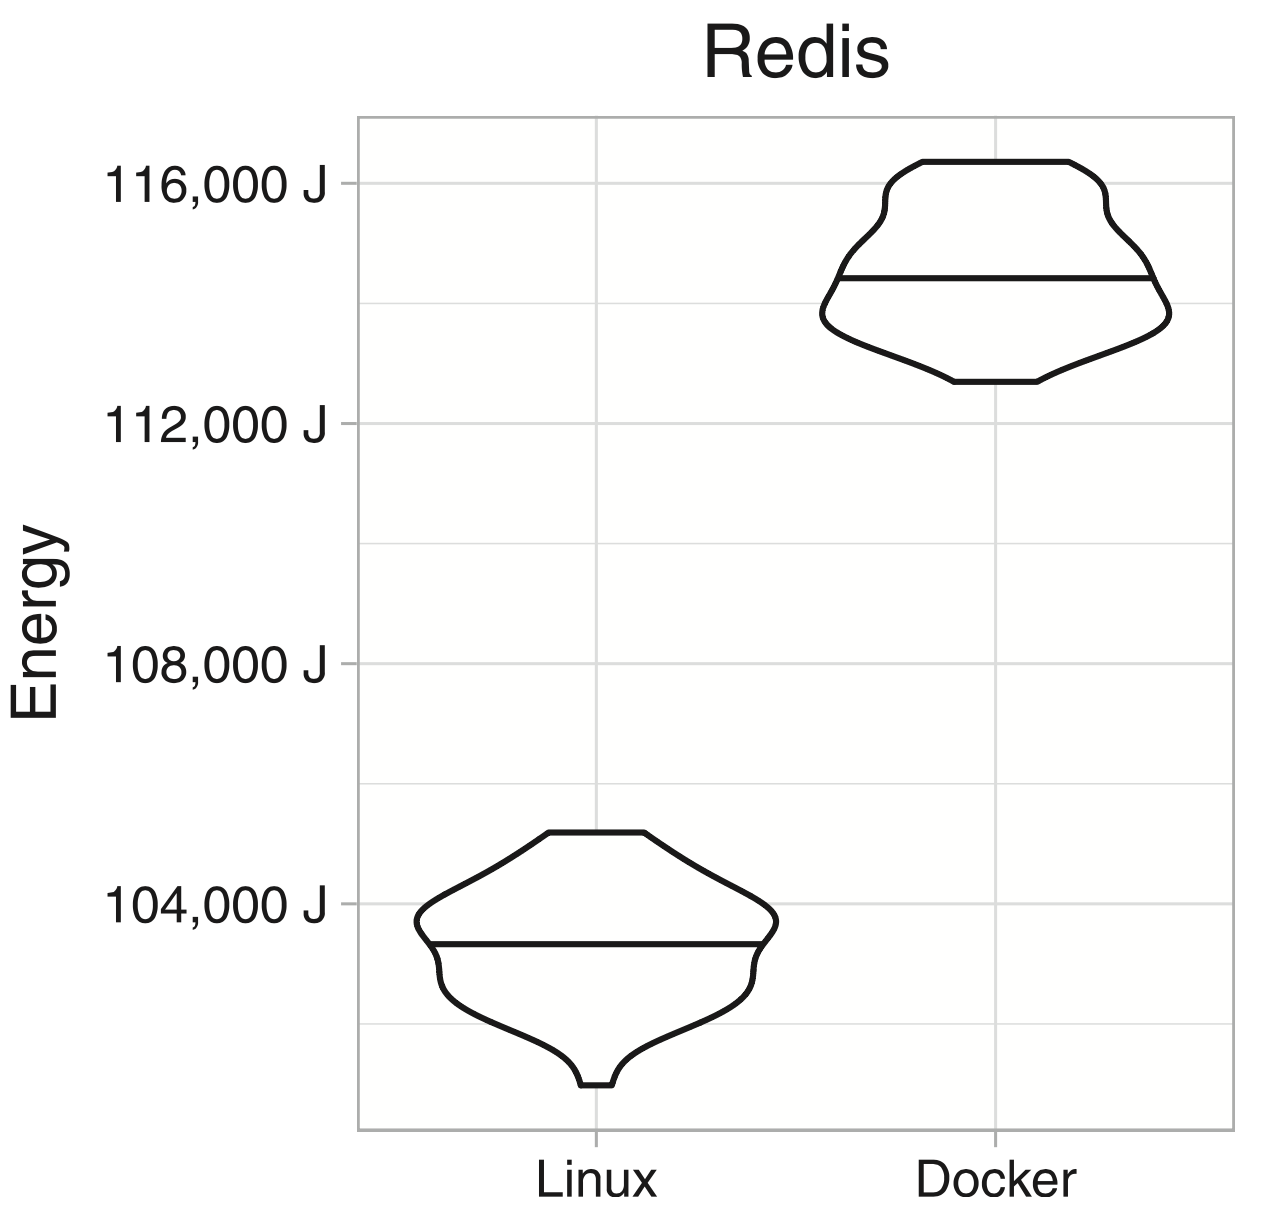
\includegraphics[width=.5\linewidth]{imgs/docker_vs_vm_energy_paper/reddis_energy}
    \caption{Execution time \& energy consumption of Redis with and without Docker~\cite{eddie_antonio_santos_how}}\label{fig:docker_reddis}
\end{figure}

As can be seen, the introduction of the supervisor has increased the impact of Docker on energy that will be applied equitably to all experiments.
Therefore, when it comes to comparison analysis, it will mitigate its impact automatically.
Furthermore, because we have access to the host hardware, we do not need to worry about capturing the SUT's energy use.
As a result, we will use Docker to keep all of our tests separate, as it will make sure that they can be repeated in a clear and simple way.

\subsection{Extension}
% TODO : proofread
\subsubsection{Definition of Extention}
With the rapid evolution of the software industry, Even ensuring the reproducibility of the same research won't be enough.
Each day, new versions of the software are released, and new features are added. Even more, the goal of the research might evolve. As a result, nowadays, especially in comparative studies, it is essential to leave room for expansion.

One can extand their experiment through three axes :
\begin{itemize}
    \item \textbf{proposed solutions}: Where one will expand their research by including additional solutions and comparing them to earlier ones
    \item \textbf{evaluation criteria}: This axe's objective is to broaden the evaluation criteria to incorporate additional measures like as performance, cost, and security, among others.
    \item \textbf{benchmarks}: The purpose of this axe is to enlarge the benchmarks to include other ones in order to broaden the scope of the research.
\end{itemize}

\subsubsection{The architecture of the extension}
\begin{figure}
    \center{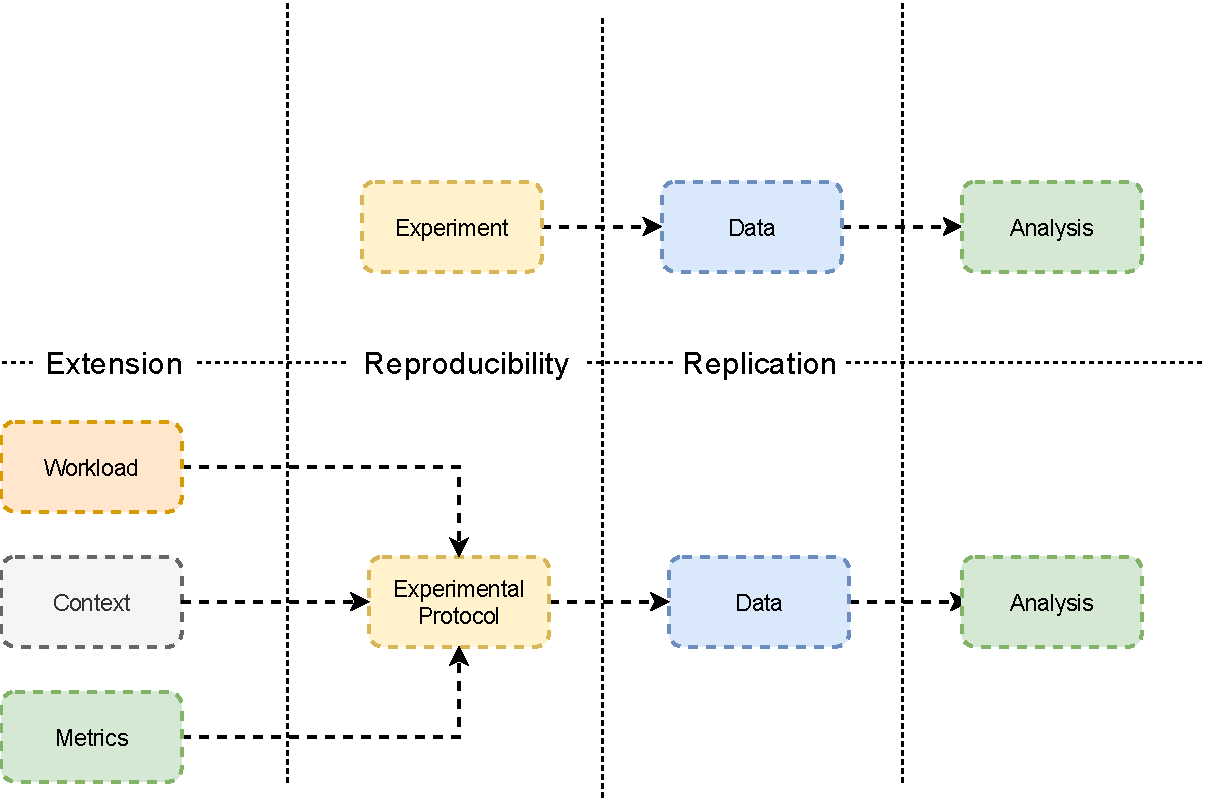
\includegraphics[width=\linewidth]{imgs/benchmarkingprotocol}}
    \caption{Benchmarking protocol}\label{fig:benchmarkingprotocol}
\end{figure}
To be able to extend the empirical experiments through these axes,
We propose to enhance the benchmarking framework suggested by the \emph{Collaboratory on Experimental Evaluation of Software and Systems in Computer Science}\footnote{\url{http://evaluate.inf.usi.ch/}}.
Instead of only presenting the four primary aspects of their guidelines that were mentioned previously in Section~\ref{sec:benchmarking_reproducibility}, we suggest an abstract model to describe an empirical experiment.
Figure~\ref{fig:benchmarkingprotocol} shows the proposed model while providing a comparaison between the existing solution and the proposed one.

The model is composed of different components that are described below,
\paragraph{Context}
The hardware and the software configuration for the actual experiment, the purpose of this part is to provide extra information to help readers have a better judgement on the results and to be able reproduce the experiment while diminishing the impact of  external factors .

\paragraph{orchestrator}

The core design of the experiment which is responsible for running the experiment regrardless of the context.
In the experiment,it is  the only component that is allowed to interact with the SUT.
The orchestrator provides three interfaces:
\begin{itemize}
    \item \emph{Workload interface} : provides a set of functions that should be implemented by the workload and called by each candidate in the experiment.This interface is responsible for extending the experiment with new benchmarks.
    \item \emph{The Observer interface}: provides a set of metrics that are collected by the orchestrator during the experiment. Implementing the observer interface allows the user to extend the experiment with new metrics.
    \item \emph{The Candidate interface} : It provides a set of functions that should be implemented by the candidate and called by the orchestrator. This interface is responsible for extending the experiment with new solutions.
\end{itemize}

\paragraph{Data}
The row data collected collected by the experiment. In ourcase it will be provided by the observator, one ore more observators can be used to collect different metrics. The purpose of this data is to ensure the \emph{replication} of the experiment which will allow the reader to perform extra analysis without rexucuting the experiment.


\paragraph{Analysis}
The final part, that should provide the set of methodes and functions used to do the empirical analysis in order to answer the research questions.



% It starts with the orchestrator is the core design of the experiment  for the coordination between the workload and the candidate, therefore it provides an interface that is implemented by each workload.
% Later this interface will be provided to each candidate by the orchestrator. Like this we will remove any bias of dependency between the workload and the candidates, which will alow us to extend both parts without any change in the code.
% Instead of retrieving the data directly from the experiment, we suggest to use an observator to allow the extension of the metrics, this observer in general should be outside the experiment to be able to gather as many informations without impacting the the code.









\subsection{Conclusion}

In this section, we addressed the first challenge of empirical research, which is the \textbf{reproducibility} of the experiments.
We started by listing the different options for encapsulating the system-under-test.
Then, we have shown that the use of VMs is not suitable for performance-related tests nor energy-related ones, while containers are a good alternative. Laterm, we discussed the pros and cons of using Docker for experiments related to energy consumption and have shown that it has a constant overhead which is self-mitigated when it comes to comparison analysis.
Lastly, we have proposed an addition to the benchmarking framework that would allow the experiment to be extended along the three axes already mentioned.



\clearpage